\documentclass[a4paper,12pt]{article}
\usepackage[T2A]{fontenc}
\usepackage[utf8]{inputenc}
\usepackage[russian]{babel}
\usepackage{amsmath}
\usepackage{amssymb}
\usepackage{graphicx}
\usepackage{booktabs}
\usepackage{geometry}
\geometry{left=20mm, right=20mm, top=20mm, bottom=20mm}

\title{Исследование характеристик случайных графов \\ для различения распределений}
\author{Куценко Дмитрий, Шатурный Алексей}
\date{2025}

\begin{document}

\maketitle

\section{Постановка задачи}
В данной работе рассматривается задача классификации двух пар параметрических распределений ($\text{Laplace}(0, \beta)$ с $\text{Normal}(0, \sigma^2)$ и $\text{Pareto}(\alpha)$ с $\text{Exp}(\lambda)$)  с использованием конструкций случайных графов. Основная цель - исследовать, как числовые характеристики графов, построенных на выборках из этих распределений, зависят от параметров распределений и могут быть использованы для построения статистического критерия.

\subsection{Математическая формулировка}
Пусть задана выборка $\hat{\Xi} = (\xi_1, \ldots, \xi_n)$ независимых реализаций случайной величины $\xi$. Требуется проверить две гипотезы:
\begin{itemize}
    \item $H_0: \xi \sim \mathcal{N}(0, \sigma^2)$ - нормальное распределение (для Алексея $\text{Pareto}(\alpha)$)
    \item $H_1: \xi \sim \text{Laplace}(0, \beta)$ - распределение Лапласа (для Алексея $\text{Exp}(\lambda)$)
\end{itemize}

Для решения задачи используются две конструкции случайных графов:
\begin{enumerate}
    \item \textbf{KNN-граф} $\mathcal{GK}(\hat{\Xi}, k)$:
    \begin{itemize}
        \item Вершины: индексы наблюдений $V = \{1, \ldots, n\}$
        \item Рёбра: $(i,j) \in E$ если $\xi_j \in \text{KNN}(\xi_i, k)$ или $\xi_i \in \text{KNN}(\xi_j, k)$
    \end{itemize}
    
    \item \textbf{Дистанционный граф} $\mathcal{GD}(\hat{\Xi}, d)$:
    \begin{itemize}
        \item Вершины: индексы наблюдений $V = \{1, \ldots, n\}$
        \item Рёбра: $(i,j) \in E$ если $|\xi_i - \xi_j| \leq d$
    \end{itemize}
\end{enumerate}

\section{Исследование характеристик графов}
В первой части работы исследовалось поведение числовых характеристик графов в зависимости от параметров распределений.

\subsection{Используемые характеристики}
Для анализа были выбраны следующие характеристики графов:
\begin{enumerate}
    \item Для пары из распределений $\text{Normal}$ и $\text{Laplace}$
    \begin{itemize}
        \item Число треугольников - для KNN-графа
        \item Хроматическое число - для дистанционного графа
    \end{itemize}

    \item Для пары из распределений $\text{Pareto}$ и $\text{Exp}$
    \begin{itemize}
        \item Число компонент связности - для KNN-графа
        \item Размер минимального кликового покрытия - для дистанционного графа
    \end{itemize}
\end{enumerate}

\subsection{Методология исследования}
Для каждого типа графа и характеристики проводилось:
\begin{enumerate}
    \item Фиксация размера выборки $n$ и параметра построения графа ($k$ или $d$)
    \item Вариация параметра распределения:
    \begin{itemize}
        \item Для нормального: $\sigma \in [0.5, 8.0]$
        \item Для Лапласа: $\beta \in [0.5, 8.0]$
    \end{itemize}
    \item Для каждого набора параметров выполнялось 100 симуляций Монте-Карло
    \item Усреднение значений характеристики по симуляциям
\end{enumerate}

\subsection{Результаты}

\subsubsection{Зависимость характеристик от параметра $\sigma$ нормального распределения}
Ниже представлены зависимости характеристик от параметров распределений при фиксированных $n=100$, $k=5$, $d=1.5$.

\begin{center}
% 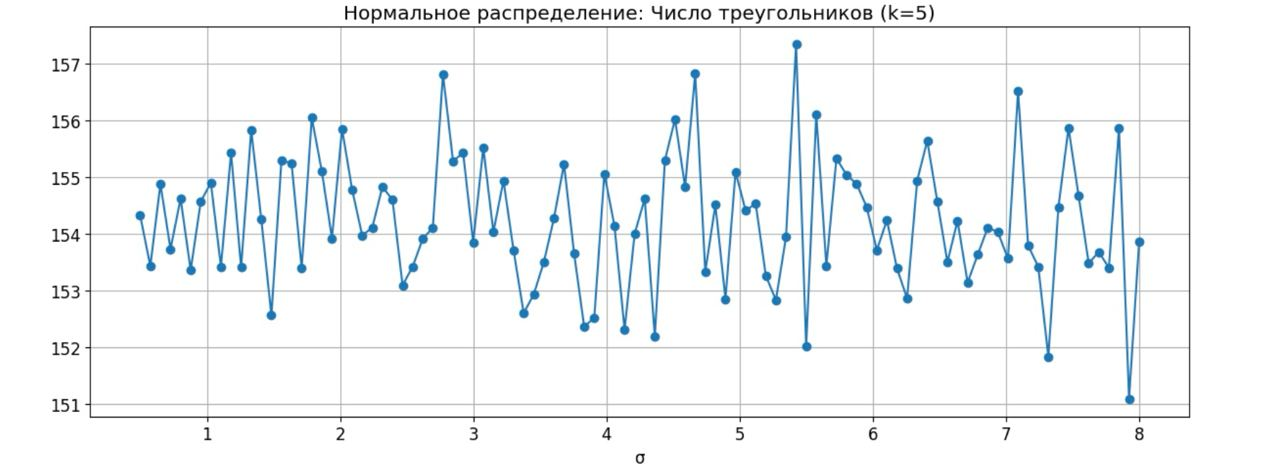
\includegraphics[width=0.8\textwidth]{images/number_triangles_normal.png}
% 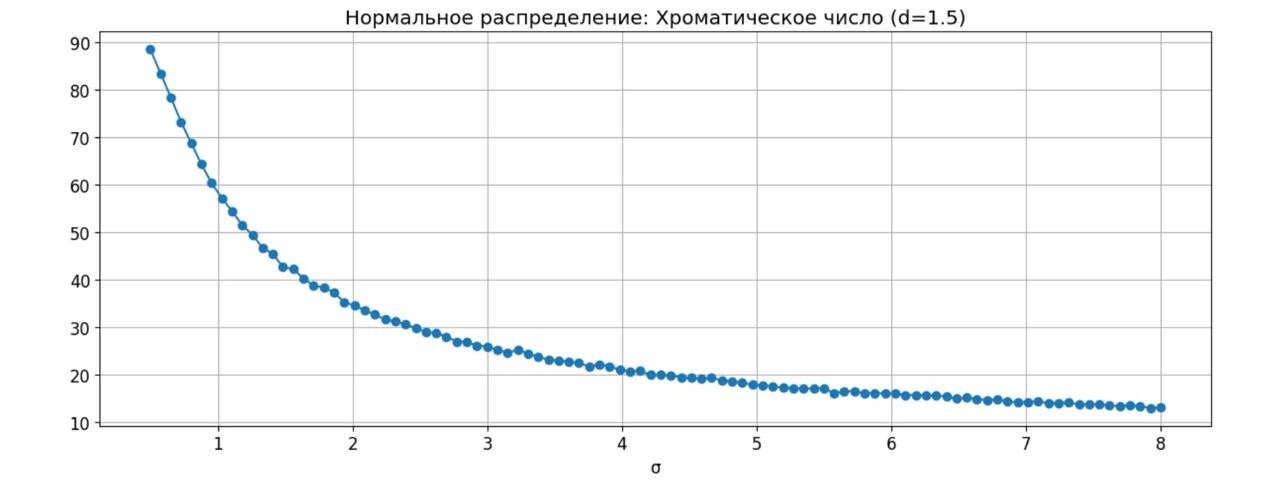
\includegraphics[width=0.8\textwidth]{images/chromatic_number_normal.png}
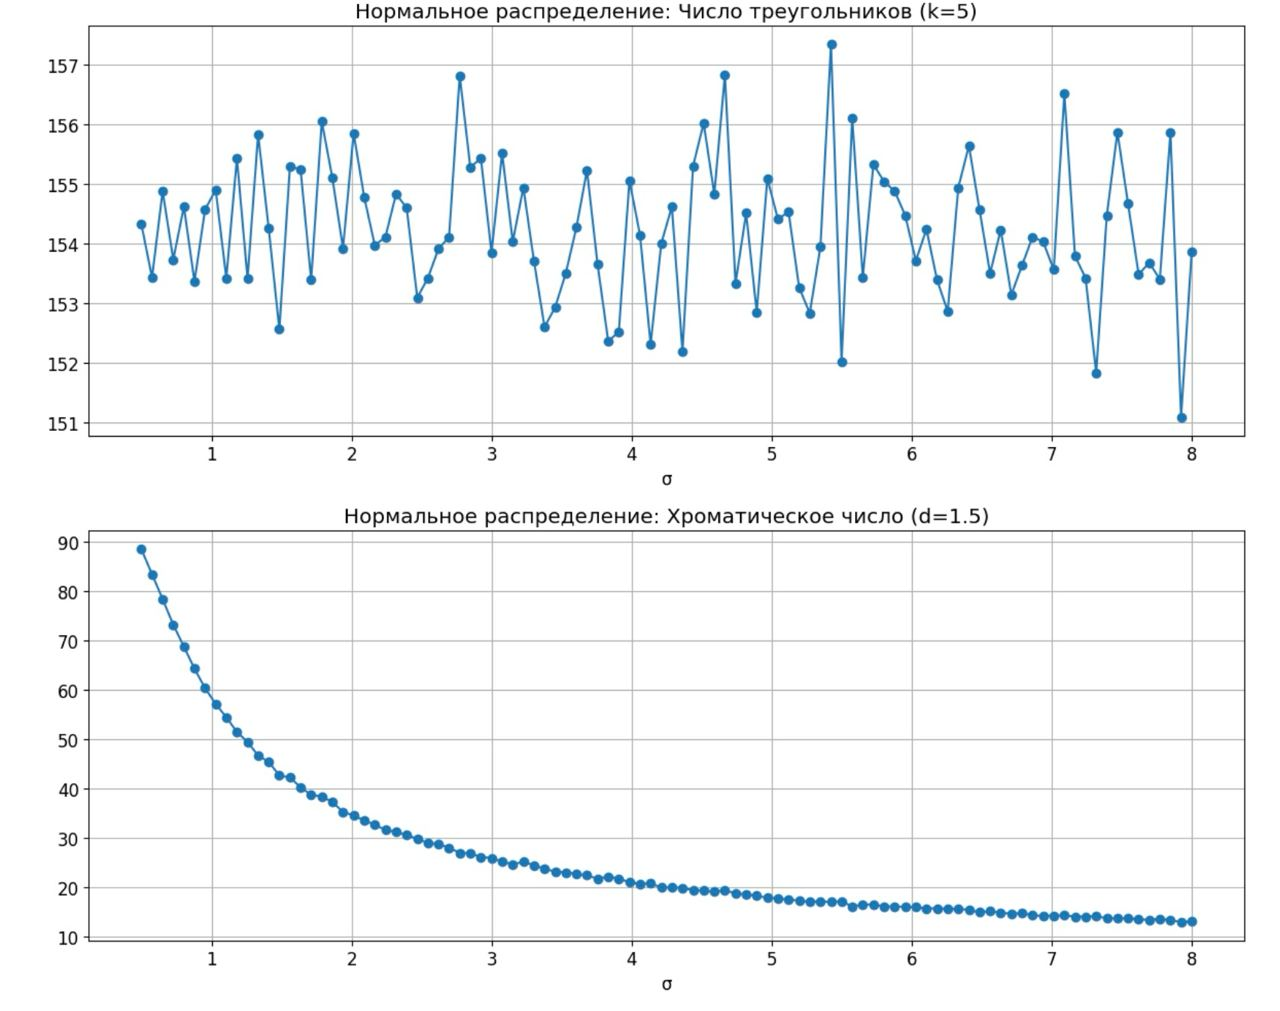
\includegraphics[width=0.8\textwidth]{images/normal_sigmas.png}
\end{center}

Основные наблюдения:
\begin{itemize}
    \item \textbf{Число треугольников (KNN-граф)}:
    \begin{itemize}
        \item Тяжело установить явную зависимость числа треугольников в получаемом KNN-графе в зависимости от параметра $\sigma$ нашего распределения. В среднем количество треугольников колеблется около 154
    \end{itemize}
    
    \item \textbf{Хроматическое число (дистанционный граф)}:
    \begin{itemize}
        \item Резко убывает с ростом $\sigma$
        \item Объяснение: вероятно увеличение разброса приводит к разрежению графа
    \end{itemize}
\end{itemize}


\subsubsection{Зависимость характеристик от параметра $\beta$ распределения Лапласа}

\begin{center}
    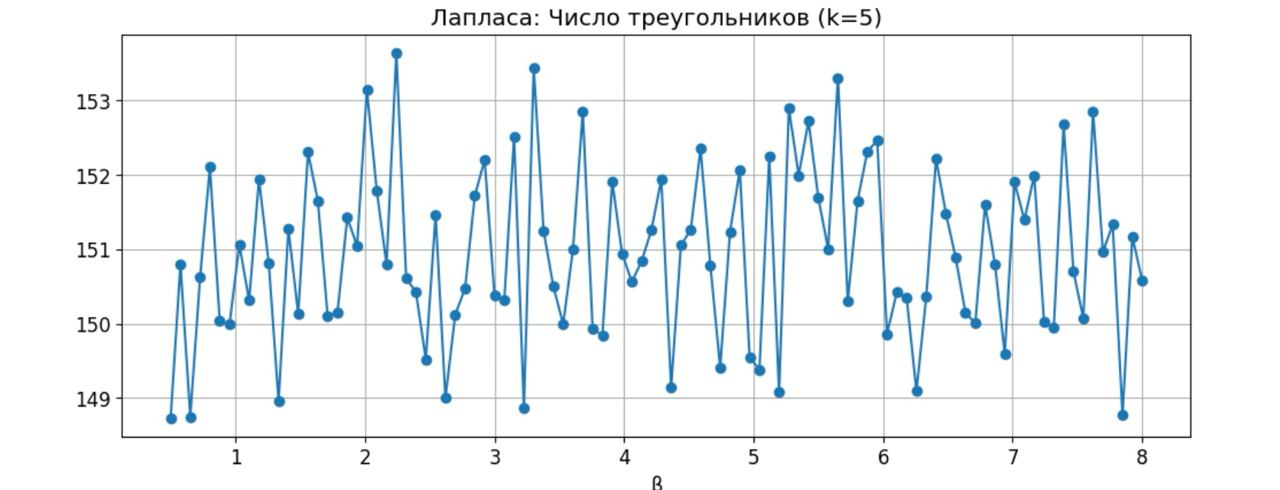
\includegraphics[width=0.8\textwidth]{images/number_triangles_laplace.png}
    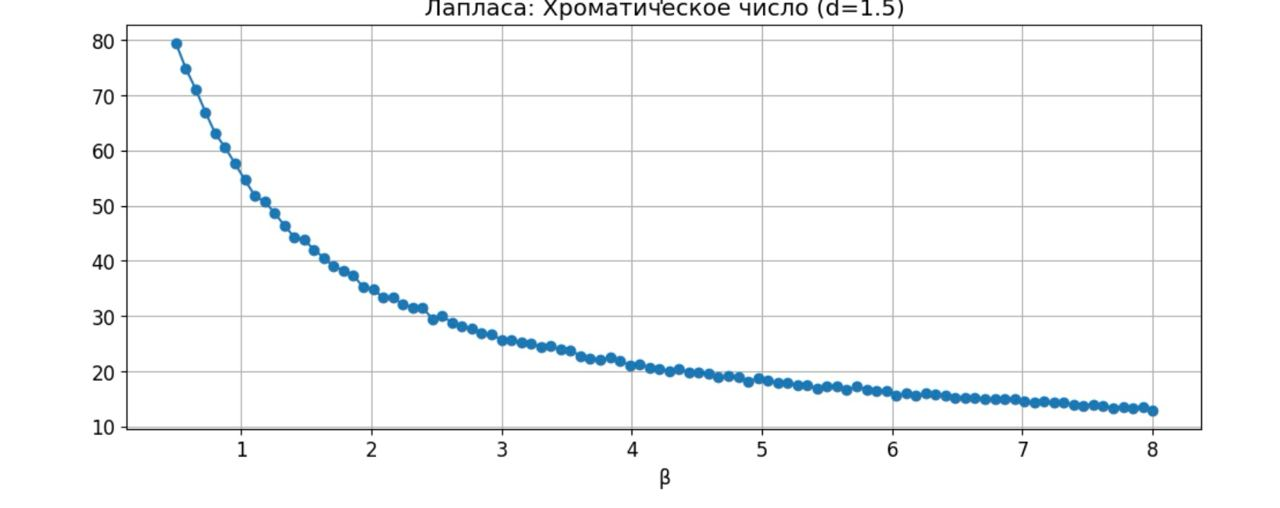
\includegraphics[width=0.8\textwidth]{images/chromatric_number_laplace.png}
\end{center}

Можем наблюдать ситуацию, похожую на нормальное распределение -- видна явная зависимость хроматического числа от параметра $\beta$, в то время как число треугольников в KNN-графе колеблется вокруг значения 151



\subsubsection{Зависимость характеристик от параметров $\lambda$ экспоненциального распределения и $\alpha$ распределения Парето}

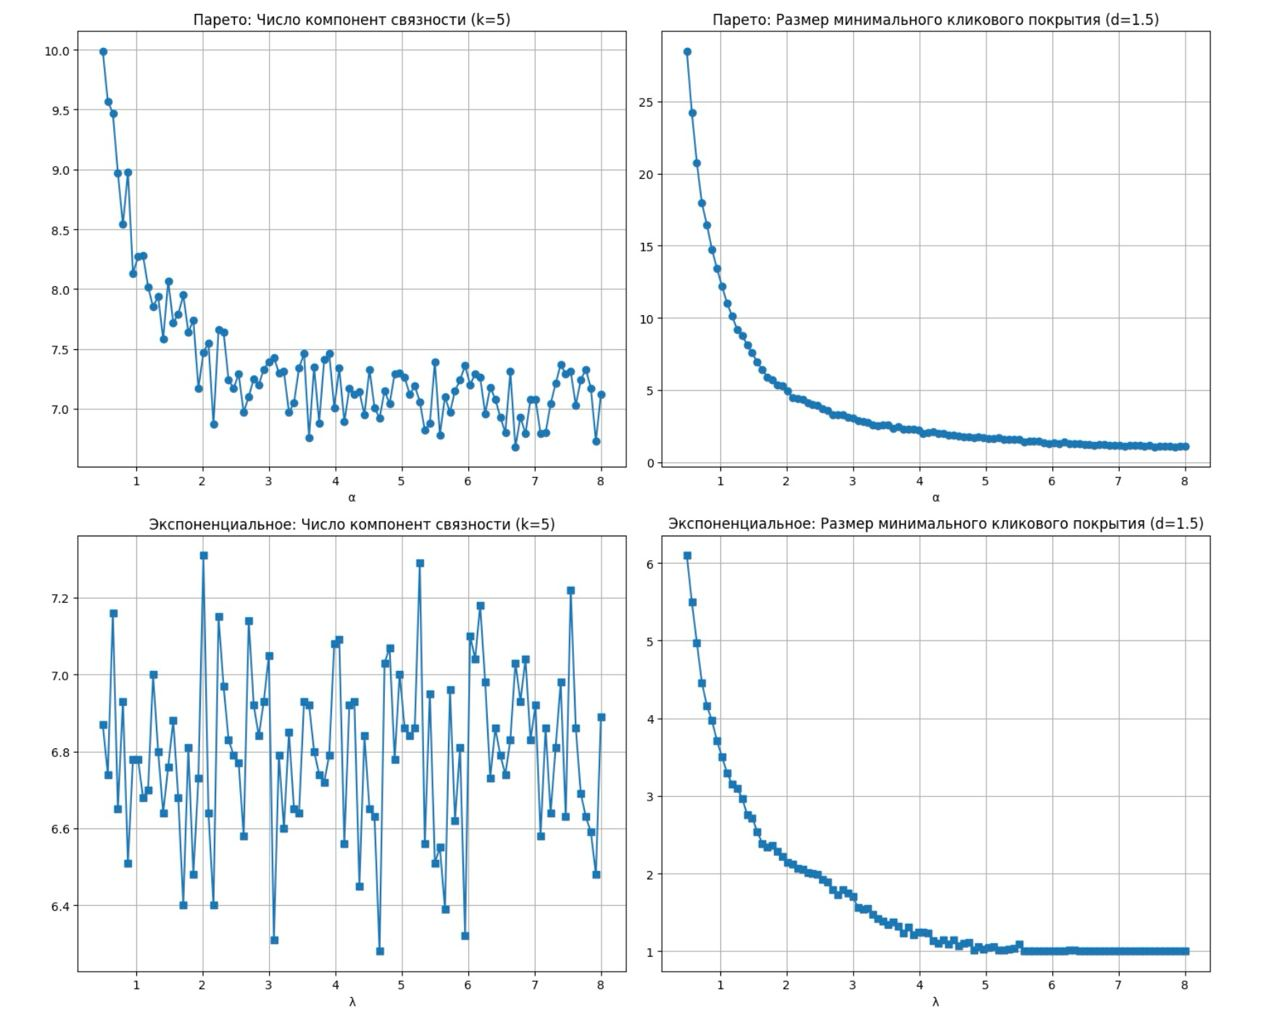
\includegraphics[width=1\textwidth]{images/exp_pareto_graph_1.png}
Основные наблюдения:
\begin{enumerate}
    \item Аналогично паре из нормального распределения и распределения Лапласа числовая характеристика дистанционного графа выглядит более информативной и менее шумной

    \item С увеличением $\lambda$ и $\alpha$ для обоих распределения размер минимального кликового покрытия дистанционного графа резко падает
\end{enumerate}



\subsubsection{Исследование поведения числовых характеристик в зависимости от параметров процедуры построения графа и размера выборки при фиксированных параметрах распределений}
% На рис. \ref{fig:size_dependency} показана зависимость характеристик от размера выборки при фиксированных параметрах распределений ($\sigma=1.0$, $\beta=\sqrt{1/2}$) и параметрах графов ($k=5$, $d=1.5$).
Будем симулировать выборки при фиксированных параметрах распределений:
\begin{enumerate}
    \item $\text{Laplace}\left( 0, \sqrt{\frac{1}{2}}\right)$
    \item $\text{Normal} \left(0, 1 \right)$
    \item $\text{Pareto} (3)$
    \item $\text{Exp} \left(\frac{2}{\sqrt{3}} \right)$
\end{enumerate}
Рассмотрим следующие параметры процедуры построения графов
\begin{enumerate}
    \item $k = 1, 2, 3, ..., 20$
    \item $d \in [1, 3]$
    \item $n = 50, 100, 200, 500$
\begin{center}
    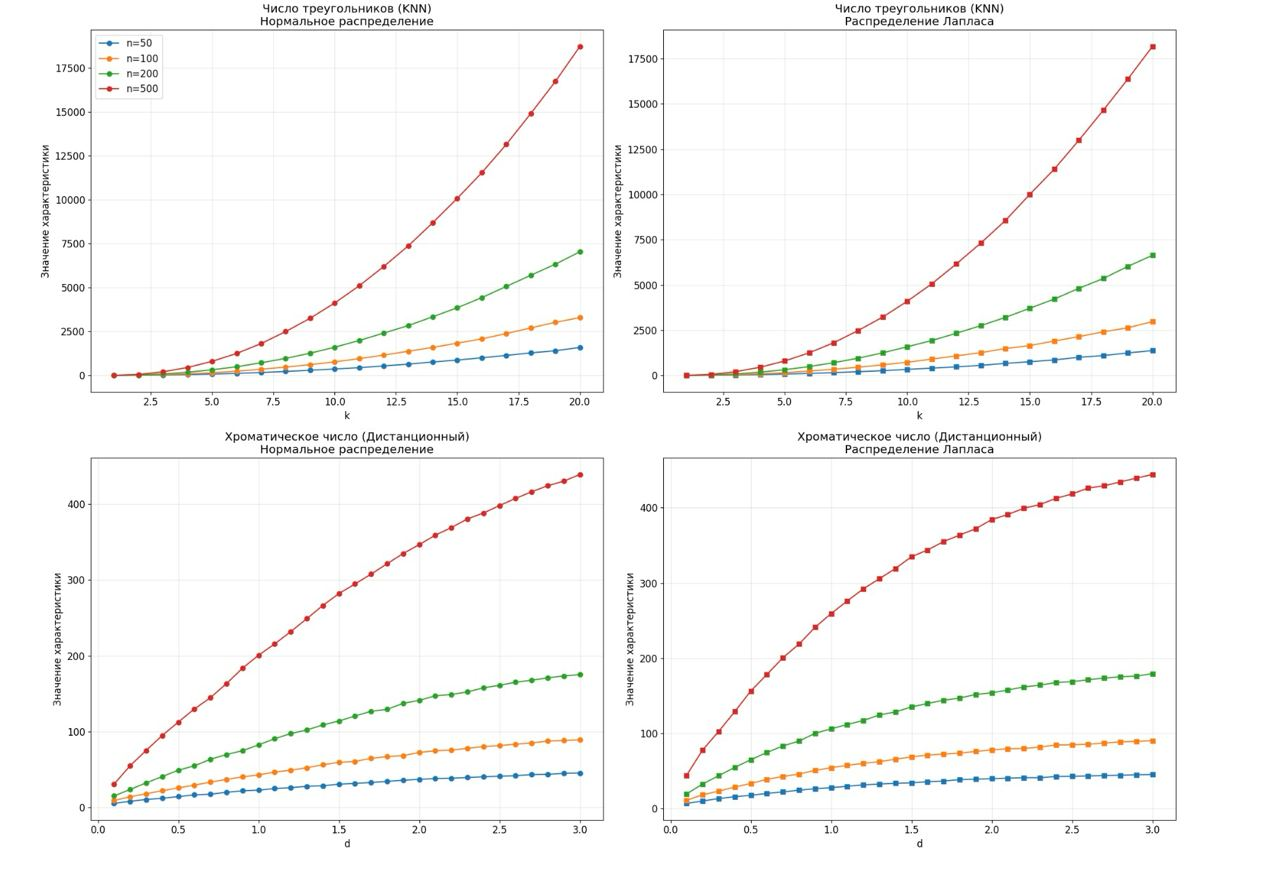
\includegraphics[width=1\textwidth]{images/diff_params_laplace_normal.png}
    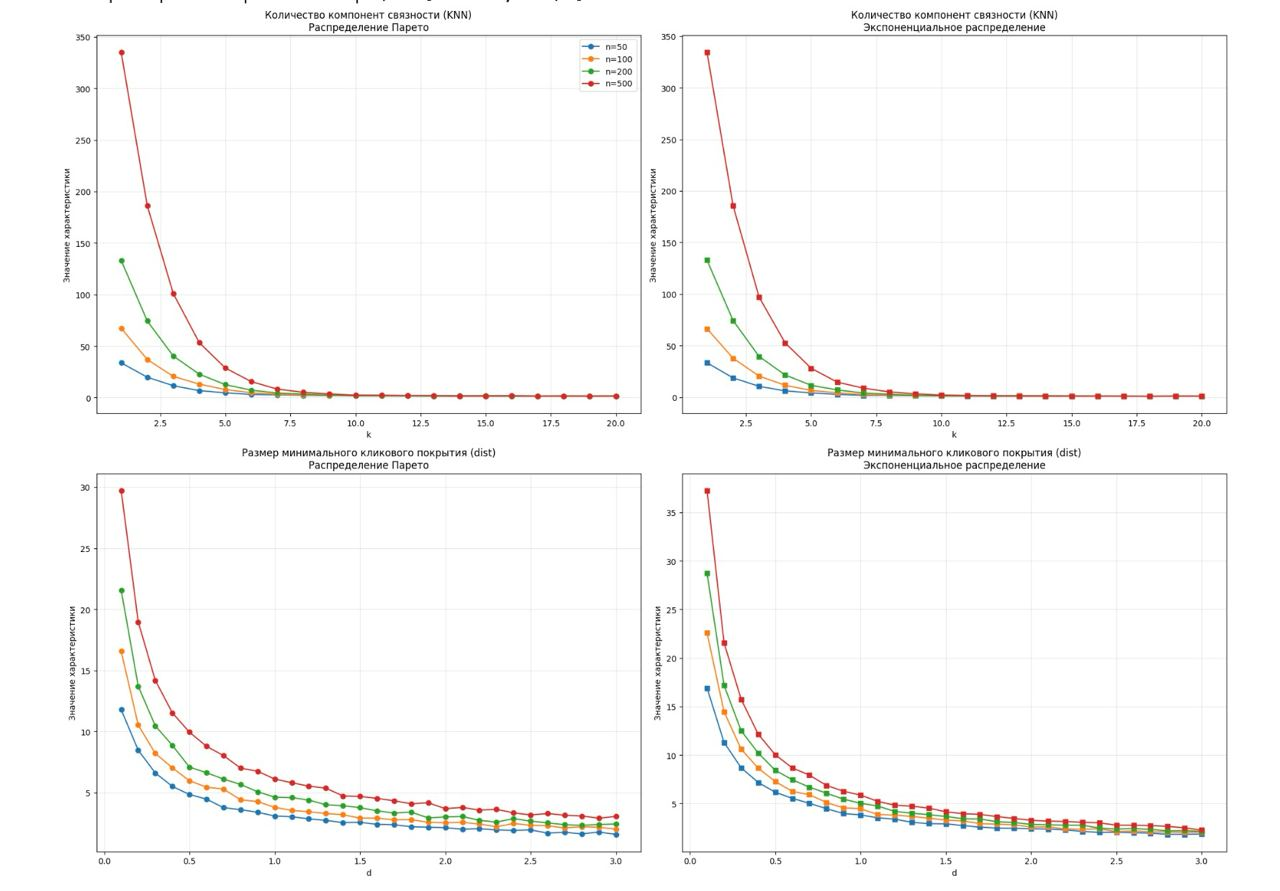
\includegraphics[width=1\textwidth]{images/diff_params_pareto_exp.png}
\end{center}
\end{enumerate}


Основные наблюдения:
\begin{enumerate}
    \item При исследовании пары из нормального распределения и распределения Лапласа было установлено, что при увеличении параметров $k$ и $d$ вне зависимости от величины $n$, обе числовые характеристики получаемых случайных графов растут.

    \item В паре из распределения Парето и экспоненциального распределения наоборот при увеличении параметров $k$ и $d$ исследуемые числовые характеристики падали

    \item В обоих случаях логично с увеличением размера выборок (то есть параметра $n$) значение числовых характеристик росло, но характер роста (или наоборот падения) оставался прежним
\end{enumerate}

\subsubsection{Построение критических областей}

\section{Заключение первой части}
Проведенное исследование показало:
\begin{enumerate}
    \item Числовые характеристики случайных графов чувствительны к параметрам распределений

    \item Пронаблюдали род зависимости каждой из выбранных числовых характеристик KNN-графа и дистанционного графа в зависимости от различных параметров распределений
    
    \item Более информативную и явную зависимость удалось выявить при исследовании дистанционных графов
    \begin{itemize}
        \item Для пары $\text{Laplace}$ и $\text{Normal}$ хорошо показало себя хроматическое число

        \item Для пары $\text{Pareto}$ и $\text{Exp}$ хорошо показал себя размер минимального кликового покрытия
    \end{itemize}
\end{enumerate}

\section{Применение нескольких характеристик для проверки гипотезы}

\subsubsection{Выбор модели случайного графа}
По итогам исследования поведения числовых характеристик при изменении параметров распределений и параметров процедуры построения графа было принято решение работать именно с дистанционным графом, так как числовые характеристики дистанционного графа проявляли себя как более информативные.


\subsubsection{Фиксирование параметров распределений и параметров процедуры построения графа}
\begin{enumerate}
    \item $\text{Laplace}\left( 0, \sqrt{\frac{1}{2}}\right)$
    \item $\text{Normal} \left(0, 1 \right)$
    \item $\text{Pareto} (3)$
    \item $\text{Exp} \left(\frac{2}{\sqrt{3}} \right)$
    \item $d = 1.5$
\end{enumerate}

\subsubsection{Построение обучающего набора данных}
\begin{enumerate}
    \item Построим набор данных из 5000 объектов для $n = 25$ (В таком наборе данных поровну объектов для каждого из распределений в паре -- по 2500)

    \item Набор данных из 5000 объектов для $n = 100$

    \item Набор данных из 200 объектов для $n = 500$
\end{enumerate}

\subsubsection{Выбор моделей машинного обучения}
Для классификации распределений для обоих пар использовались 3 классических алгоритма классификации, позволяющих интерпретировать важность каждого из признаков:
\begin{enumerate}
    \item Логистическая регрессия
    \item Случайный лес
    \item Градиентный бустинг
\end{enumerate}

\subsubsection{Оценка метрик качества классификации нормального распределения и распределения Лапласа}
\begin{center}
    \includegraphics[width=1\textwidth]{images/laplace_normal_classification.png}
\end{center}

\subsubsection{Оценка метрик качества классификации экспоненциального распределения и распределения Парето}
\begin{center}
    \includegraphics[width=1\textwidth]{images/pareto_exp_classification.png}
\end{center}



Можем видеть, что при увеличении параметра $n$ -- размера выборок, метрики качества классификации растут. Выбранные модели очень хорошо справляются с поставленной задачей

\subsubsection{Исследование важности характеристик, как признаков классификации нормального распределения и распределения Лапласа}

\begin{center}
    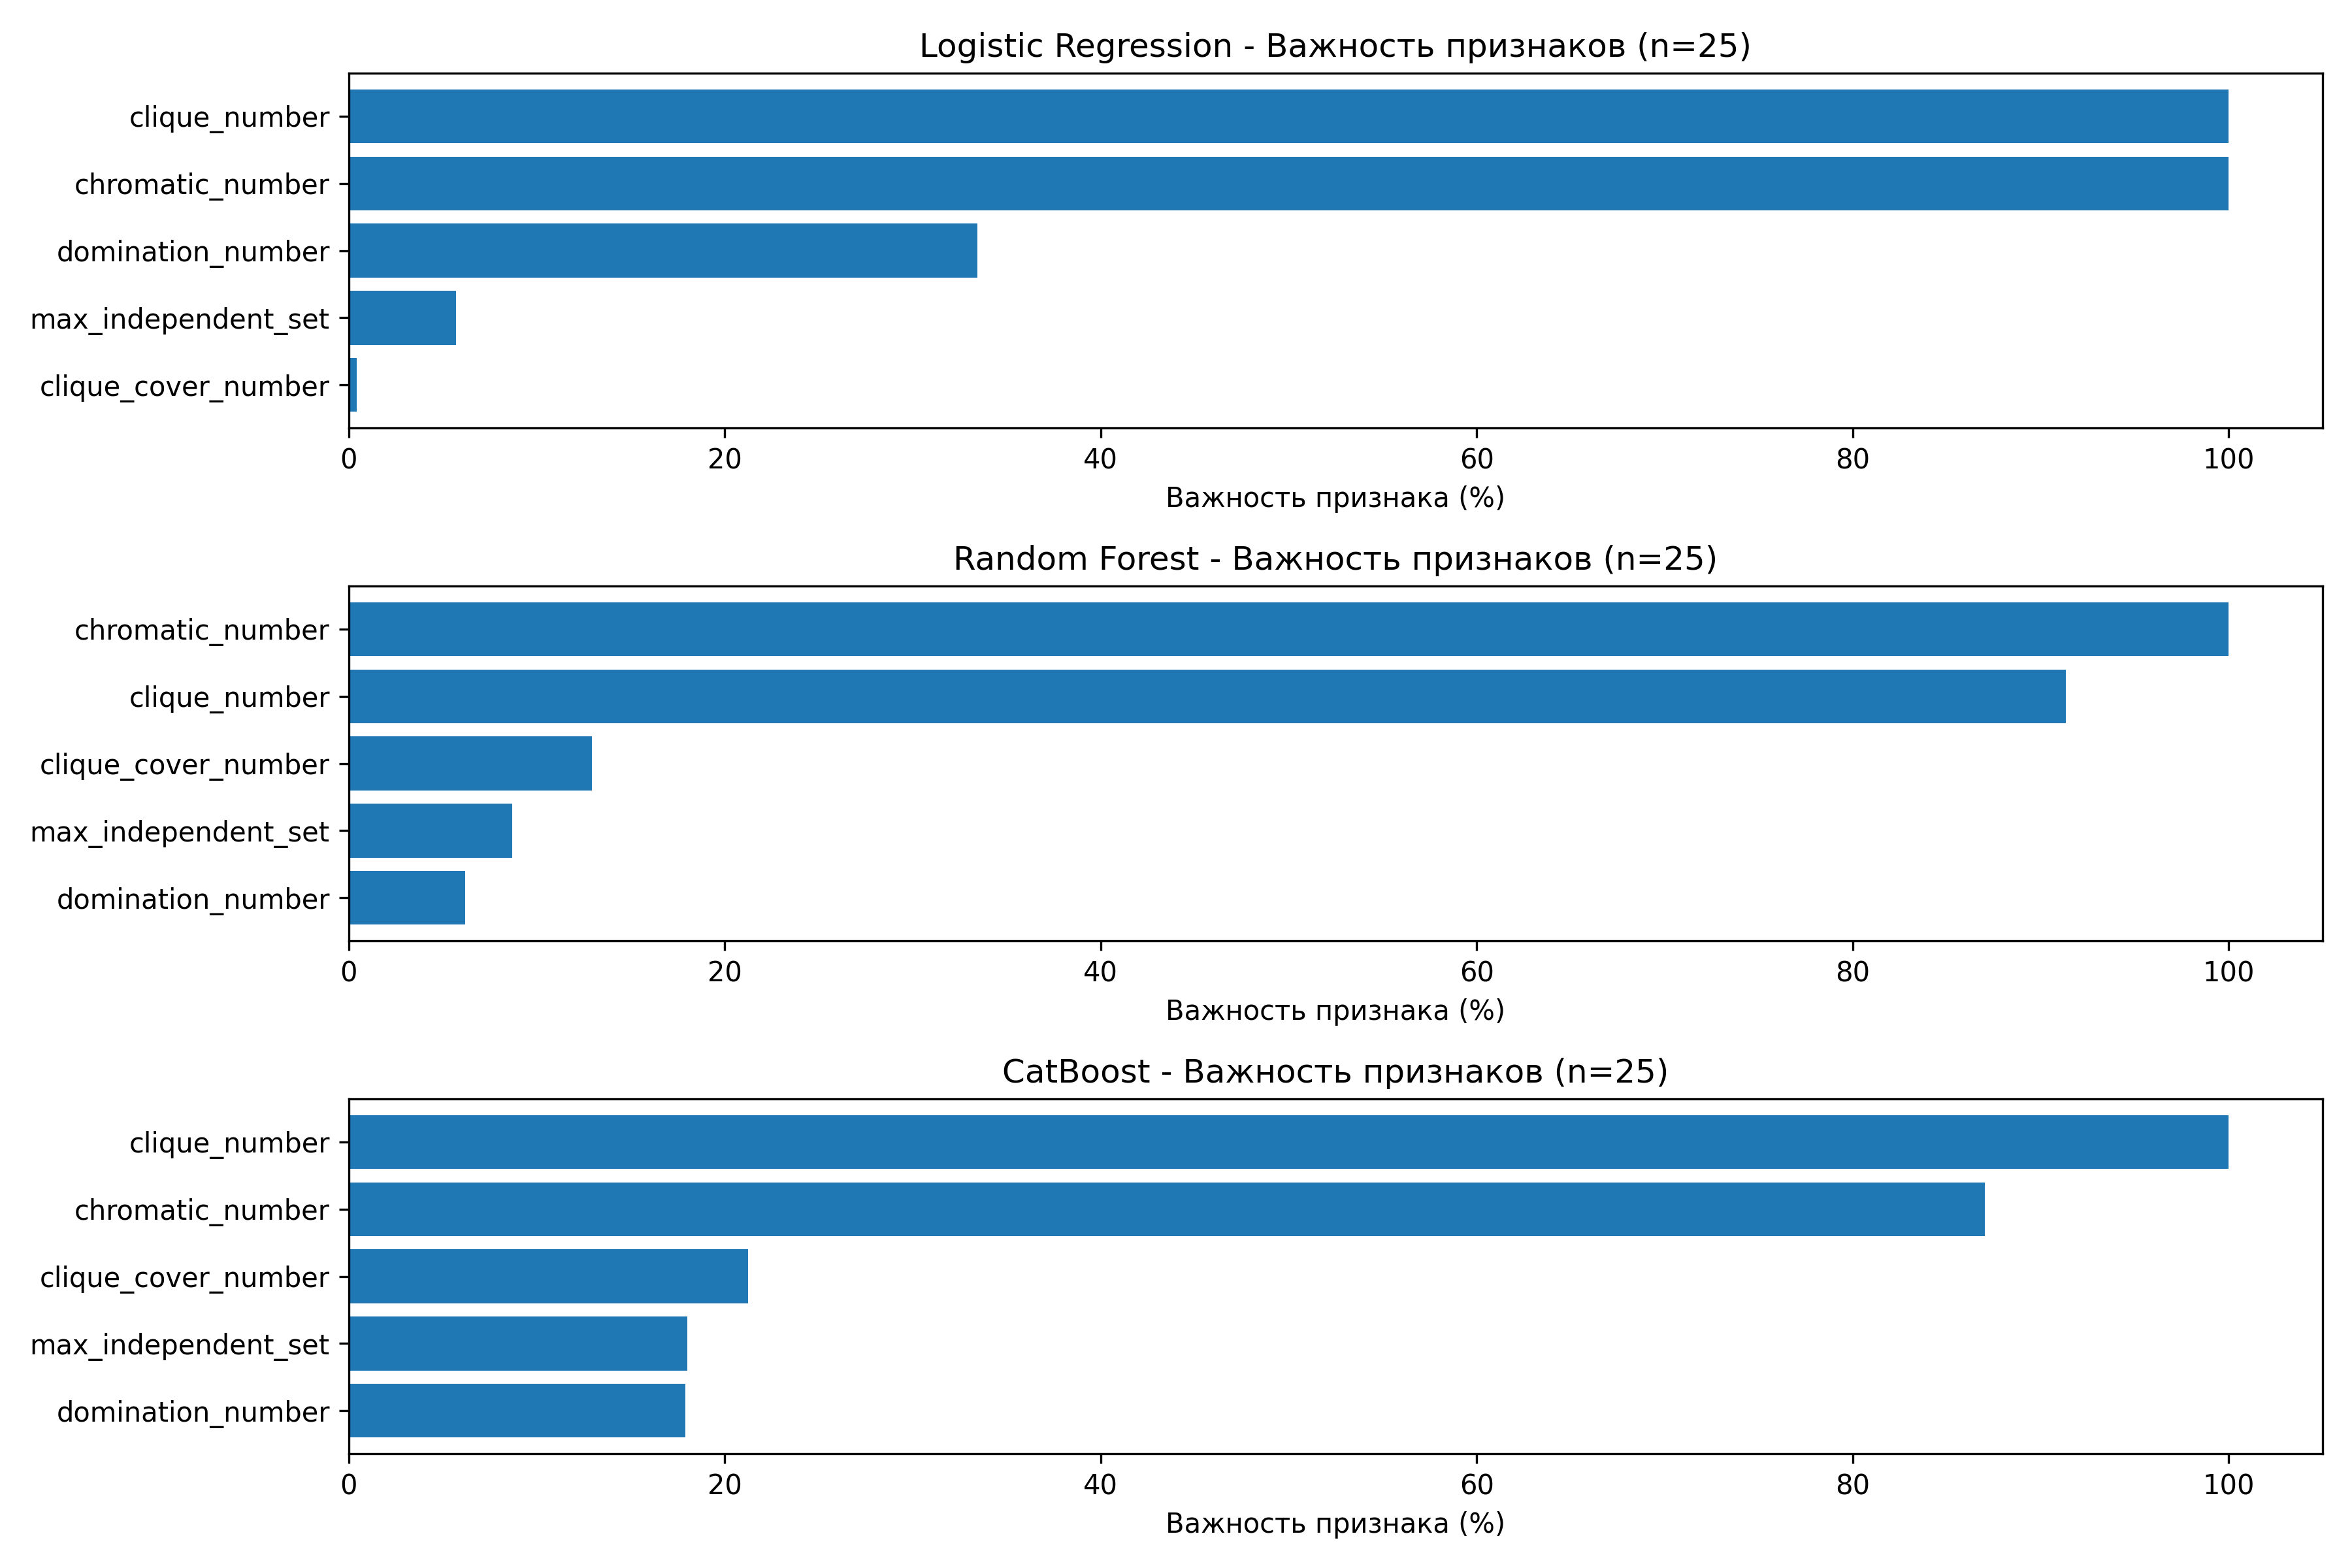
\includegraphics[width=0.8\textwidth]{images/feature_importance_n25.png}
    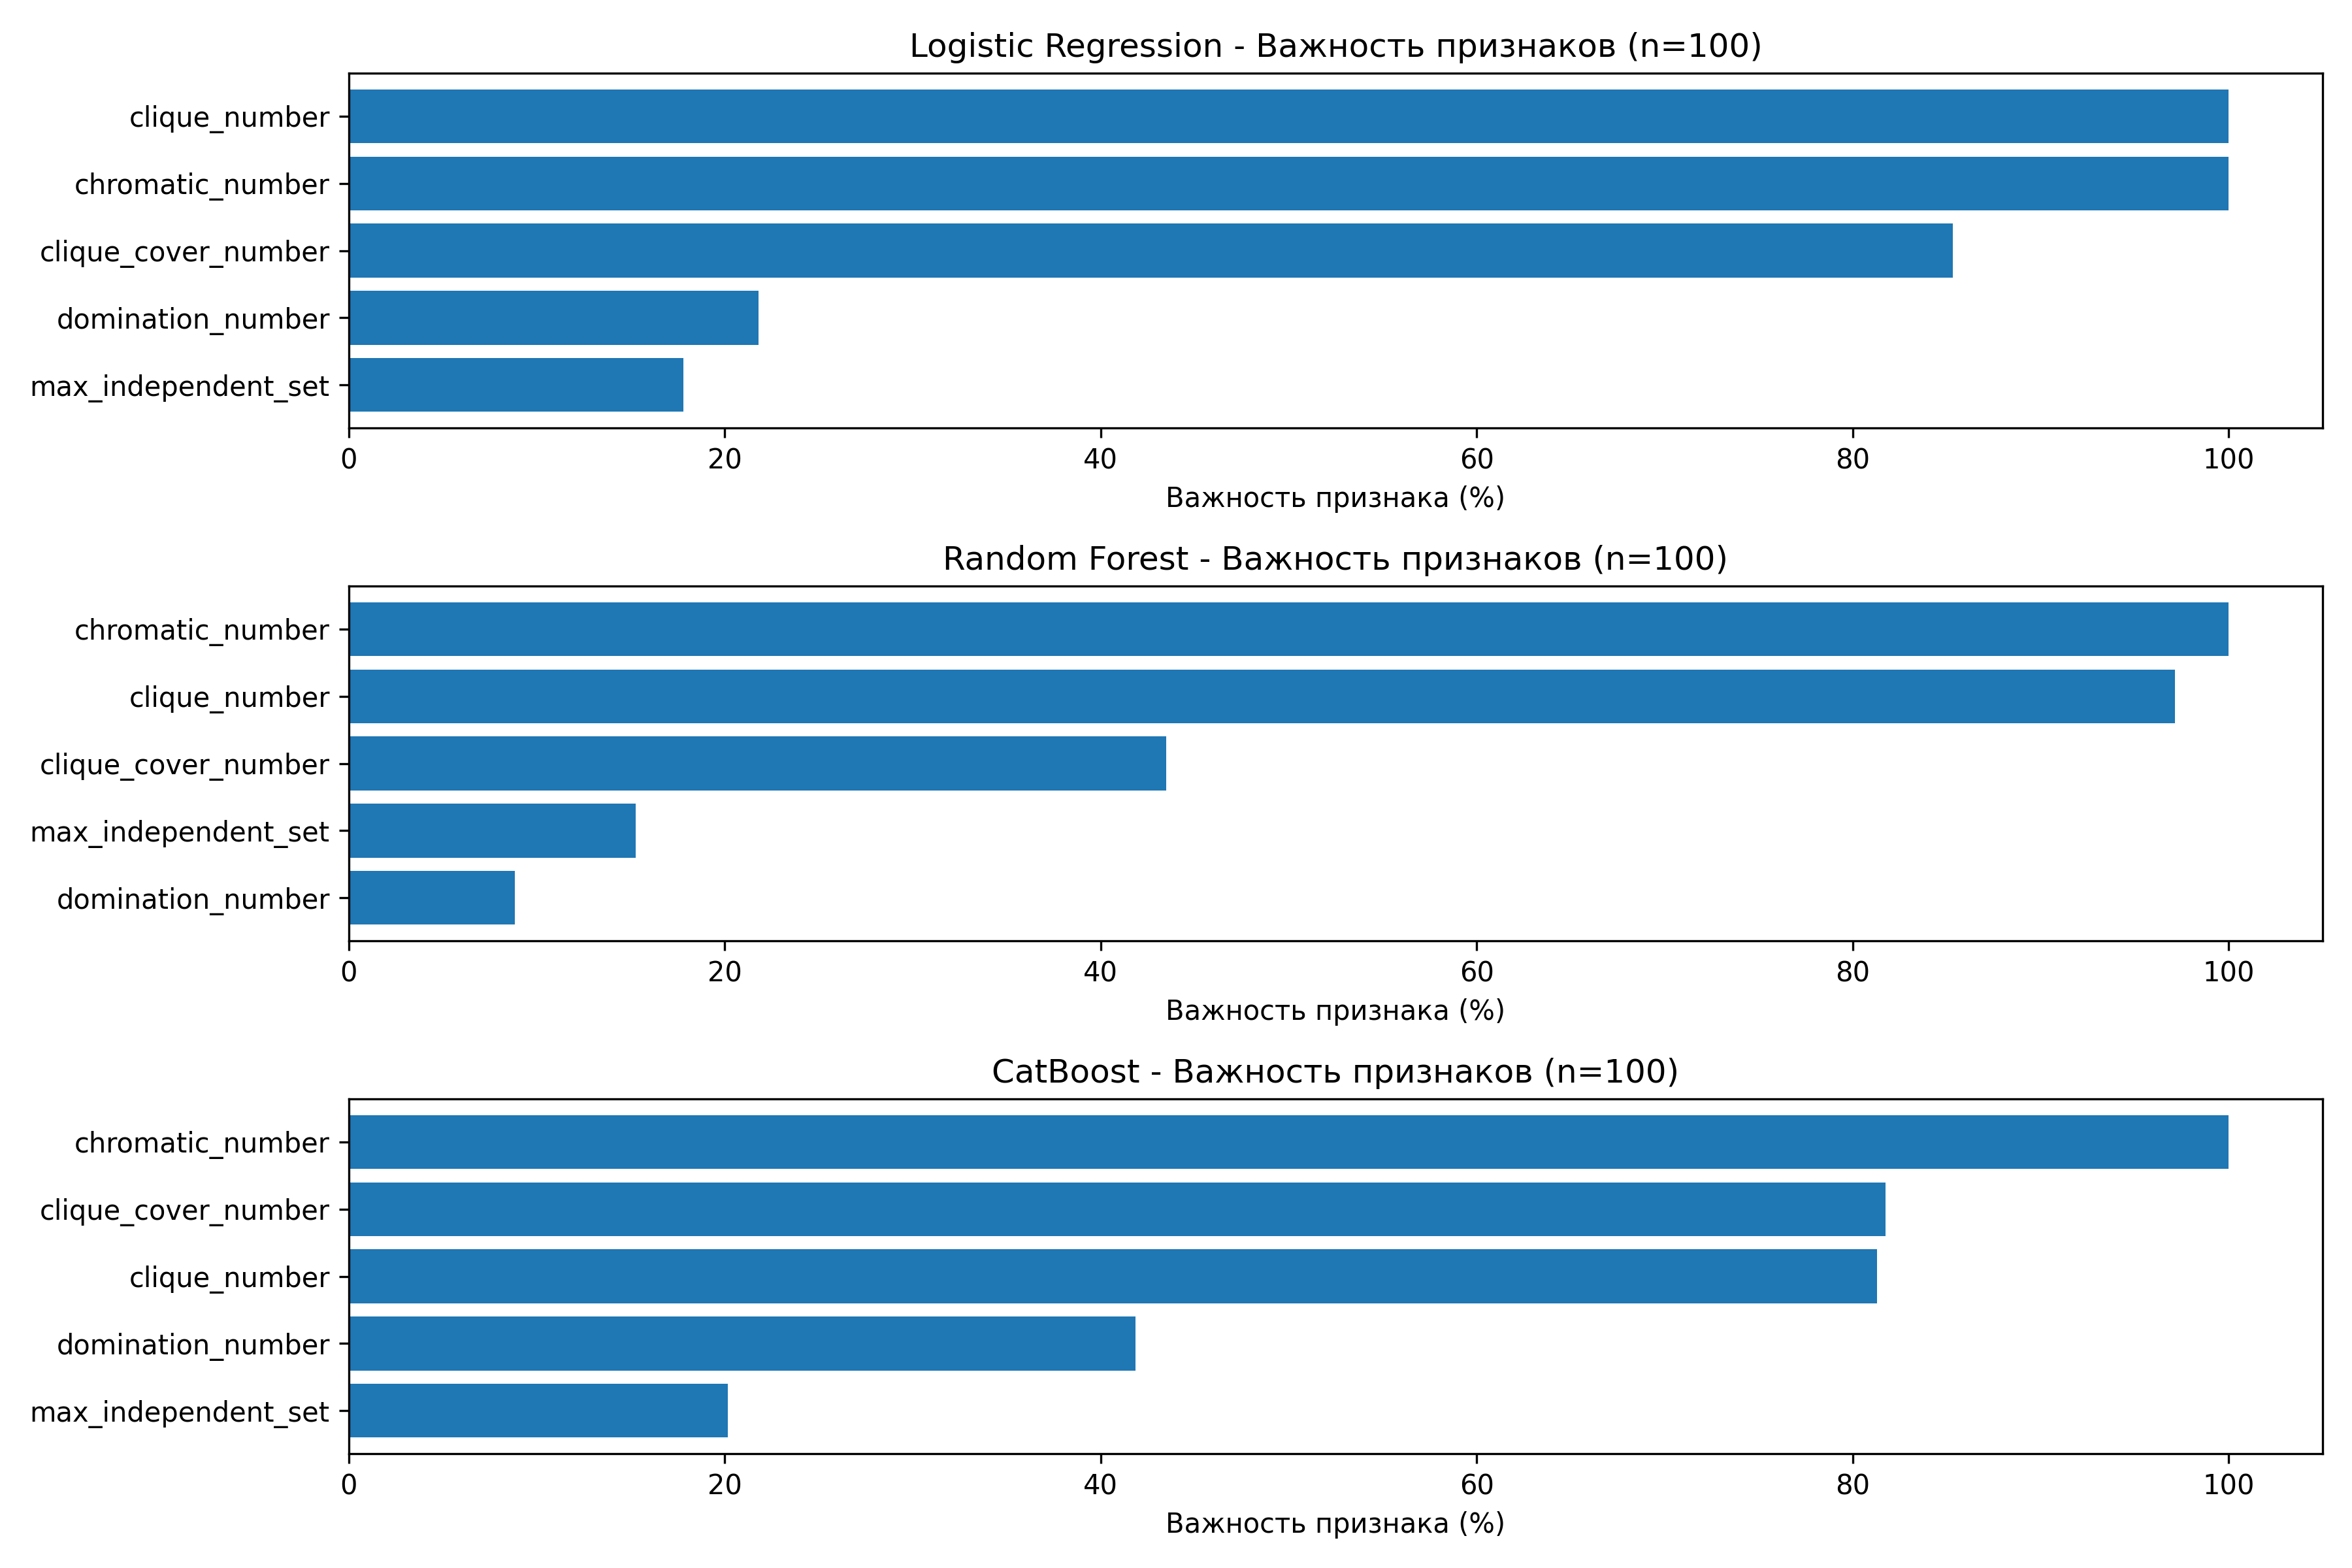
\includegraphics[width=0.8\textwidth]{images/feature_importance_n100.png}
    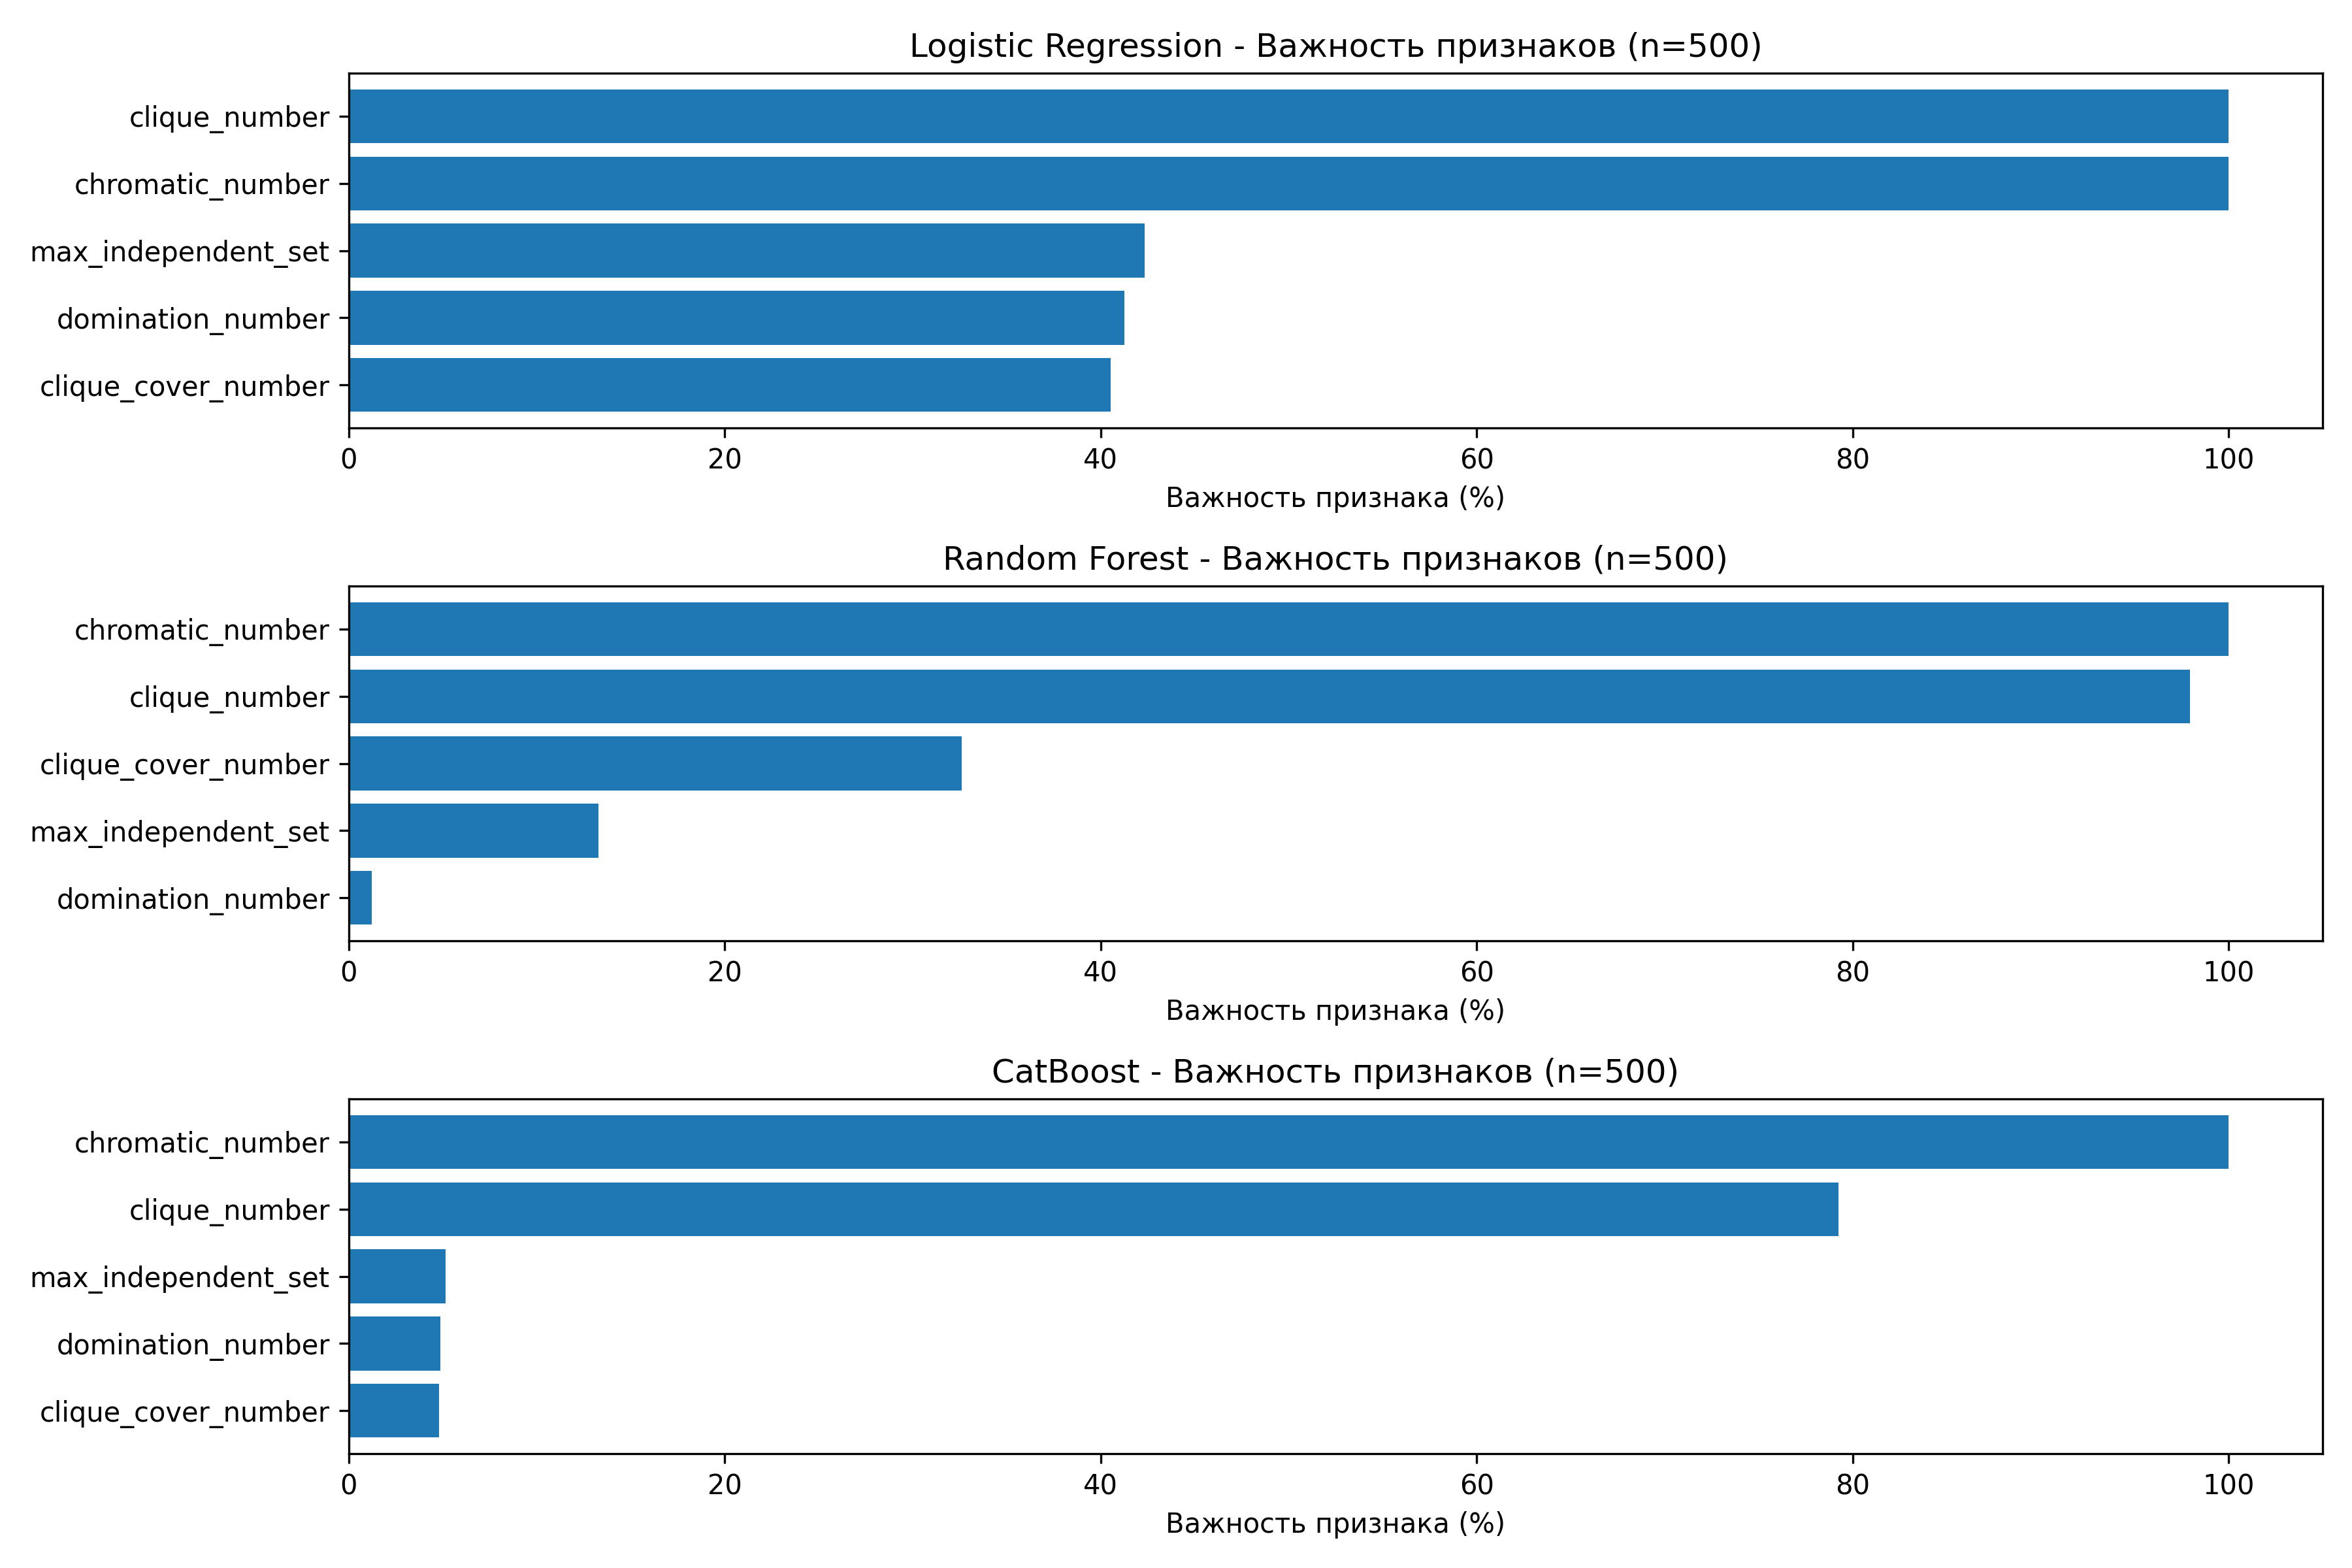
\includegraphics[width=0.8\textwidth]{images/feature_importance_n500.png}
\end{center}
Как мы можем видеть для каждого из наших алгоритмов самыми важными признаками оказались кликовое число и хроматическое число. Также при изменении величины $n$ можем заметить небольшие изменения важности остальных признаков.

\subsubsection{Выводы о вероятности ошибки первого рода и мощности полученных статистических критериев для классификации нормального распределения и распределения Лапласа}
\begin{center}
    \includegraphics[width=0.8\textwidth]{images/laplace_normal_stat_analysis.png}
\end{center}

Получили хорошие значения мощности построенных критериев и довольно низкие вероятности ошибки первого рода


\subsubsection{Выводы о вероятности ошибки первого рода и мощности полученных статистических критериев для классификации экспоненциального распределения и распределения Парето}
\begin{center}
    \includegraphics[width=0.8\textwidth]{images/pareto_exp_stat_analys.png}
\end{center}
Общие выводы:
\begin{enumerate}
    \item Для второй пары распределений мощность полученных критериев оказалась еще лучше, что делает построенные статистические критерии еще более эффективными, чем построенный в первой части. 

    \item Можем заметить, что при увеличении $n$ логично росла мощность каждого из критериев и падала вероятность ошибки первого рода

\end{enumerate}

\end{document}